\documentclass[border=2pt]{standalone}
\usepackage[dvipsnames,svgnames,x11names]{xcolor}
\usepackage{tikz}
\usetikzlibrary{arrows.meta,backgrounds,fit}
\begin{document}
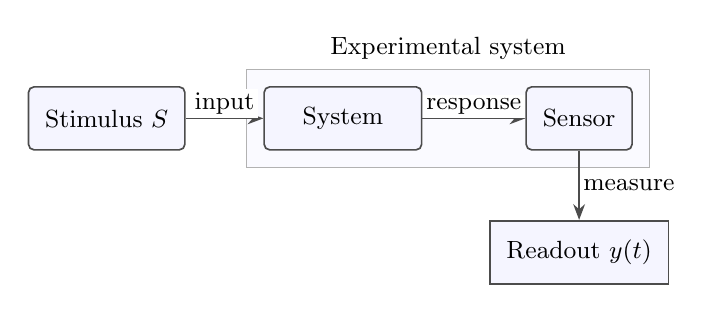
\begin{tikzpicture}[font=\small,>=Stealth]
\node[rectangle,rounded corners=2pt,fill=blue!4,draw=black!70,text=black,line width=0.6pt,minimum height=8mm,inner xsep=6pt,inner ysep=4pt,align=center] (source) at (0,0) {Stimulus $S$};
\node[rectangle,rounded corners=2pt,fill=blue!4,draw=black!70,text=black,line width=0.6pt,minimum height=8mm,inner xsep=6pt,inner ysep=4pt,align=center,minimum width=20mm] (system) at (3,0) {System};
\node[rectangle,rounded corners=2pt,fill=blue!4,draw=black!70,text=black,line width=0.6pt,minimum height=8mm,inner xsep=6pt,inner ysep=4pt,align=center] (sensor) at (6,0) {Sensor};
\node[rectangle,fill=blue!4,draw=black!70,text=black,line width=0.6pt,minimum height=8mm,inner xsep=6pt,inner ysep=4pt,align=center] (readout) at (6,-1.7) {Readout $y(t)$};
\begin{scope}[on background layer]
\node[fit=(system)(sensor),inner sep=6pt,fill=blue!2,draw=black!30,line width=0.45pt,label={[font=\small]above:{Experimental system}}] (apparatus) {};
\end{scope}
\draw[->,draw=black!70,line width=0.6pt] (source) -- node[pos=0.5,above,fill=white,inner sep=1.2pt] {input} (system);
\draw[->,draw=black!70,line width=0.6pt] (system) -- node[pos=0.5,above,fill=white,inner sep=1.2pt] {response} (sensor);
\draw[->,draw=black!70,line width=0.6pt] (sensor) -- node[pos=0.5,right,fill=white,inner sep=1.2pt] {measure} (readout);
\end{tikzpicture}
\end{document}
